% Created 2018-09-12 Mit 22:49
% Intended LaTeX compiler: pdflatex
\documentclass[a4paper,twoside]{article}
\usepackage[utf8]{inputenc}
\usepackage[T1]{fontenc}
\usepackage{graphicx}
\usepackage{grffile}
\usepackage{longtable}
\usepackage{wrapfig}
\usepackage{rotating}
\usepackage[normalem]{ulem}
\usepackage{amsmath}
\usepackage{textcomp}
\usepackage{amssymb}
\usepackage{capt-of}
\usepackage{hyperref}
\usepackage[T1]{fontenc}
\usepackage{lmodern}
\usepackage[margin=3.5cm]{geometry}
\usepackage[colorlinks]{hyperref}
\usepackage{pdflscape}
\author{David Pham}
\date{\today}
\title{Multivariate Time Series Error Detection}
\hypersetup{
 pdfauthor={David Pham},
 pdftitle={Multivariate Time Series Error Detection},
 pdfkeywords={},
 pdfsubject={},
 pdfcreator={Emacs 25.2.1 (Org mode 9.1.7)}, 
 pdflang={English}}
\begin{document}

\maketitle
\tableofcontents


\section{Project overview}
\label{sec:orgb24a6b5}

In the financial investment industry, the speed and the quality of processing
information is what determines if a business is sucessful or failure. In the
recent period, an emphasis has been set on machine learning algorithms for
investment strategies. One common application is the statement of the algorithms
to perform classification of companies to put them into sector.

This project aims to create and review algorithms for classifying companies by
using their share price. We will test a heuristic classifier using sample
correlation and train a deep neural network to mimic the performance the sample
correlation and study the hidden layer of the network. The projects uses data
from Quandl and SimFin.

\section{Problem Statement}
\label{sec:orgb711bc6}

The goal of this project is to create a method to embed financial time series
into a vector space and analyze qualitatively the embedding. The main
challenge to complete this projects are following.

\begin{enumerate}
\item Filter the universe of the data and acquire the data from different
sources.
\item Transform data to be usable in machine learning algorithm.
\item Create artifical data to transform the problem into a supervised learning problem.
\item Create a base model and train an advanced classifier to create the embedding.
\item Analyze briefly the embedding.
\end{enumerate}


\section{Metrics}
\label{sec:org7a915c3}

We will use the \emph{accuracy} defined as the ratio between the true positive and
negatives predictions divided by the dataset size. Or in formula

\begin{align*}
  \textrm{accuracy} = \frac{\textrm{true positives} + \textrm{true negatives}}{\textrm{sample size}}
\end{align*}

This metric is relevant because at a certain level the algorithms should be
able to assign correctly the stock price of companies to the sector of the
companies.


\section{Data}
\label{sec:org7896a9a}

The below table shows the data and how to access them.

\begin{center}
\begin{tabular}{lllr}
Type & Provider & Access to Datatest & Downloaded\\
\hline
Price & \href{https://www.quandl.com/databases/WIKIP/documentation/about}{Quandl} & \href{https://www.quandl.com/databases/WIKIP}{Quandl API} & 2018-08-21\\
Company information & \href{https://simfin.com/data/find/}{SimFin} & \href{https://s3.us-east-2.amazonaws.com/udacity-capstone-data-davidpham87/data/company\_fundamentals.csv}{S3} & 2018-08-21\\
Stocks Returns & Processed & \href{https://s3.us-east-2.amazonaws.com/udacity-capstone-data-davidpham87/data/wiki\_indices\_returns.csv}{S3} & 2018-09-11\\
Index Returns & Processed & \href{https://s3.us-east-2.amazonaws.com/udacity-capstone-data-davidpham87/data/wiki\_stocks\_returns.csv}{S3} & 2018-09-11\\
\hline
\end{tabular}
\end{center}

In our analysis, we used the closed price of the US companies provided by
Wikipedia and distributed by Quandl. As we additionally required the sectors
from the company we needed to merge it with an additional databases provided by
SimFin, which provides the taxonomy created by Global Industry Classification
Standard (GICS). We could find the sectors of \emph{726}
companies which constituted our dataset. The prices range from 1962 to 2018.

\section{Exploratory Analysis}
\label{sec:orgbb7eeb8}

\begin{figure}    
\begin{center}
  \label{fig:keras-nn}
  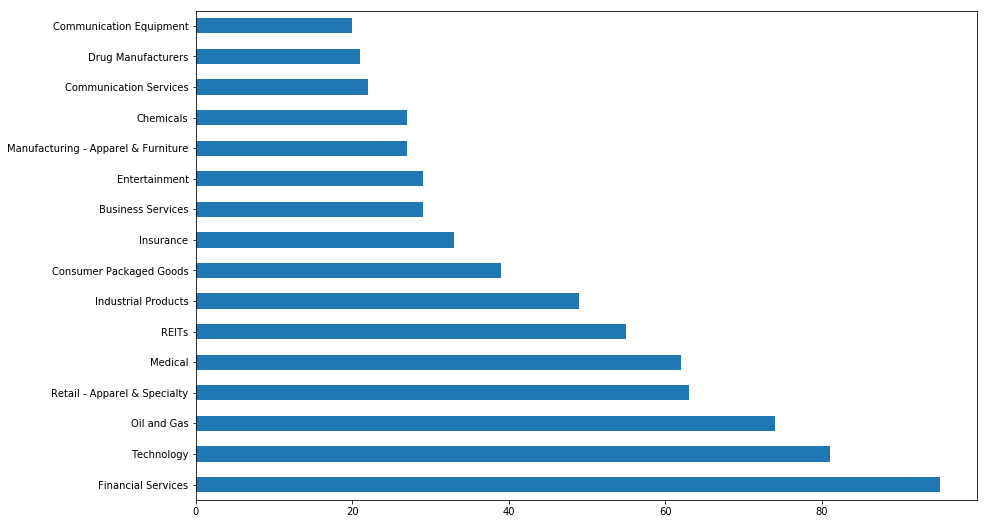
\includegraphics[width=0.95\textwidth]{figures/sectors_distribution}
  \caption{Distribution of sectors in the data.}
  \end{center}
\end{figure}

\begin{figure}    
\begin{center}
  \label{fig:keras-nn}
  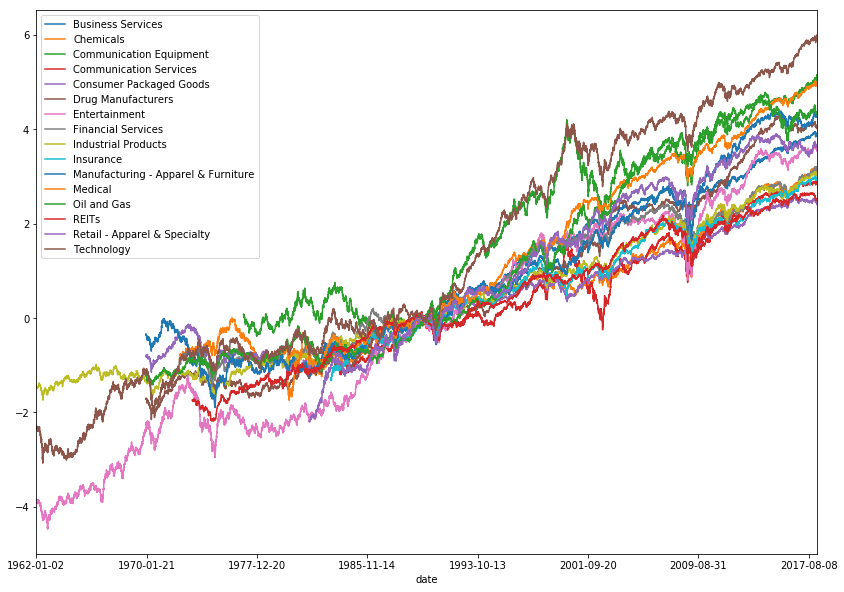
\includegraphics[width=0.95\textwidth]{figures/indexes_level}
  \caption{Synthetic indeces of sectors according to GICS. Index are set on 100 on the 1990-01-01.}
  \end{center}
\end{figure}

\section{Algorithms and Technique}
\label{sec:orga558eb8}

There is two classifiers. One is algorithmic and the is other one is based on
a \href{http://colah.github.io/posts/2014-07-Understanding-Convolutions/}{Convolutional Neural Network} (CNN). 

The first classifier computes correlations of timeseries and then assign to an
input timeseries the \emph{sector} with which it has the highest correlation. 

For two random variables \(X\) and \(Y\), with sufficient stability assumption, the
Pearson correlation is defined as

\begin{align*}
  \rho_p(X, Y) = E[XY] - E[X]E[Y] \approx \sum_{i=1}^n x_iy_i - \sum_{i=1}^nx_i\sum_{i=1}^n y_i,
\end{align*}

An interesting variant of the metric is the one applied on the rank of the \(X\)
and \(Y\). This is called the Spearman's rho coefficient and is defined as
\(\rho_s(S, R)\), where \(S\) and \(R\) are the rank variable of the \(X\) and \(Y\).
See \href{https://en.wikipedia.org/wiki/Spearman\%27s\_rank\_correlation\_coefficient}{here} for more information. The advantage of this transformation is that it
is invariant to monotonic transformation on \(X\) and \(Y\).

The second classifier use a deep neural network to create features and
representation (or state) of the inputs to be able to separate linearly all
the output sectors (or classes).

We train the neural network using \emph{Adam}, which optimize the parameters of the
network by minimizing the loss using stochastic gradient descent algorithm
which standardizes the gradient and also updates it in iteration. The batch
size was set to 32, the learning rate starts at \(0.001\) with a learning rate
scheduler that diminish the learning by \(10\%\) every 10 epochs.

\section{Methodology}
\label{sec:org6bf7dbd}

\subsection{Data preprocessing}
\label{sec:org06293d3}

From the Quandl dataset, the prepossessing involves keeping only the ticker
and the close price for as many date as possible and as many companies as
possible. Then the table is joined to the SimFin dataset containing sectors
for :insert-number-of-companies:.

In total we have, from which we can extract data.

Then the sector indices were created by averaging the daily returns of the
stocks within the sectors. The returns were floor and capped to 10\% as it is
unlikely that a indices of stocks lose or gain more than 5\% in a single
trading day.

\subsection{Implementation}
\label{sec:org90ba10c}

The implementation using Tensorflow and the keras API linked in the library.
We launched AWS server with spot instance and launched a jupyter server there
and made it accessible to our webbrowser. We develop code also in the
terminal with emacs to adapt some code.

The first step was to download the data from the several providers and to
process them. Then we needed to use several classes from keras to support
asynchronous loading of the data thanks to the \texttt{Sequence} object.

The implementation has been performed with a simple function defining the
network. We ran several experiment of the network, using adapation of
inception units and residual units, known in the neural network for images,
but they did not lead to any improvement of the model. Moreover, to avoid
overfitting, we added several batch normalization layers as well as gaussian
noise layer with a really small standard deviation. A few layers in the
network were penalized \(L_2\) regularization to insure that the features
stayed as independent as possible.


\subsection{Structure of the network}
\label{sec:org8dd4226}

The network is depicted in Figure. It is a convoluat

\begin{figure}    
\begin{center}
  \label{fig:keras-nn}
  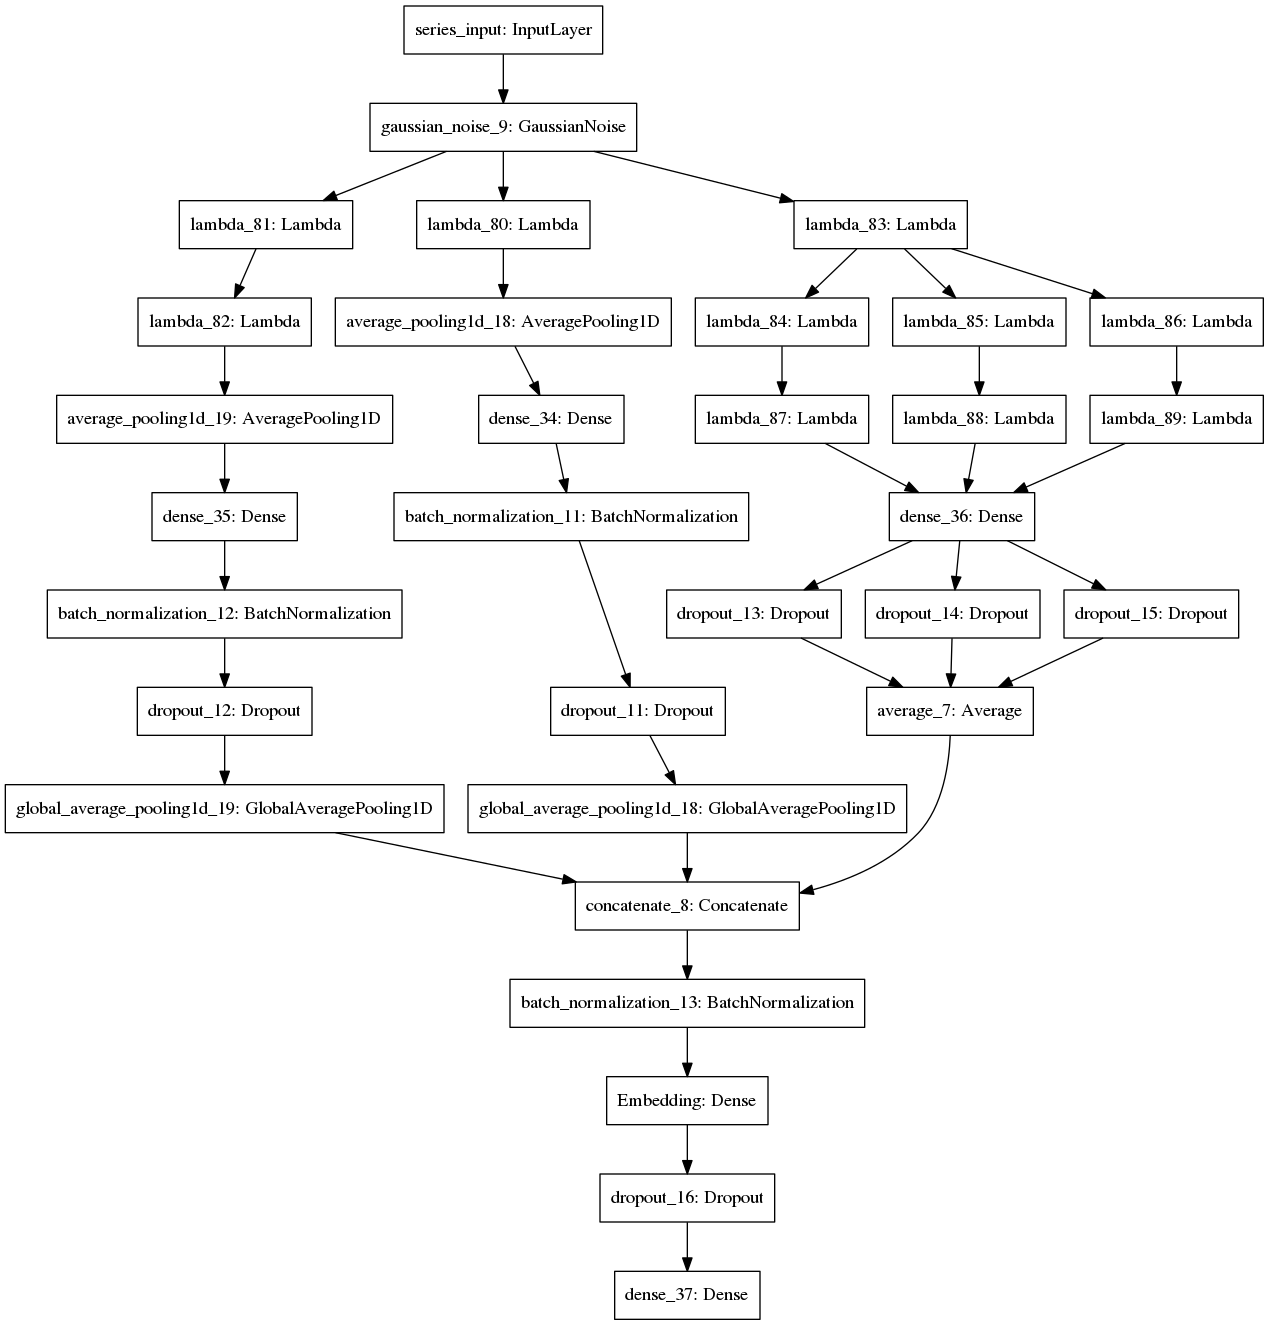
\includegraphics[height=0.95\textheight]{./figures/model_keras}
  \caption{Neural Network structure}
  \end{center}
\end{figure}





\section{Results}
\label{sec:org68e9b17}

The base model using only correlation for the period of 3 months achieves
\(59%\) accuracy in training and test set. This rather rule based method is
really good.

As for neural network model, it achieves around \(55\%\) percent accuracy on a
single observation of three months. However, we provide 25 random samples of 3
months period to the classifier, the classifier achieves \(80\%\) accuracy. As it
can be read in Table \ref{tab:orgab64cd9}.

\begin{landscape}
  \begin{figure}    
  \begin{center}
    \label{fig:confusion-matrix}
    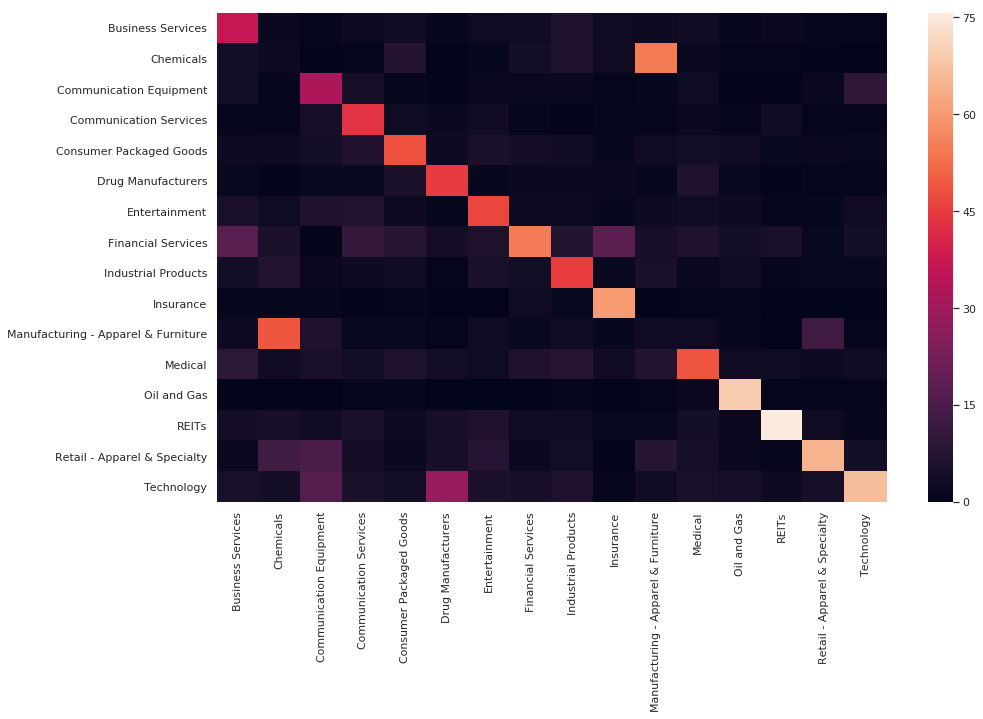
\includegraphics[height=\textheight]{./figures/confusion_matrix.png}
    \caption{Confusion matrix of our predictor.}
    \end{center}
  \end{figure}
\end{landscape}

In Figure \ref{fig:confusion-matrix}, we observe that the neural network model
classifier does a fairly good job at classifying sectors with a notable
exception of \emph{Chemicals} and \emph{Manufacturing - Apparels and Furniture}. The
reason are probably that are little data.

\begin{longtable}{|l|rrrr|}
\caption{\label{tab:orgab64cd9}
Confusion Report from the neural network classifier with resampled data.}
\\
\hline
Sector & precision & recall & f1-score & support\\
\hline
\endfirsthead
\multicolumn{5}{l}{Continued from previous page} \\
\hline

Sector & precision & recall & f1-score & support \\

\hline
\endhead
\hline\multicolumn{5}{r}{Continued on next page} \\
\endfoot
\endlastfoot
\hline
Business Services & 1.00 & 1.00 & 1.00 & 3\\
Chemicals & 0.00 & 0.00 & 0.00 & 3\\
Communication Equipment & 0.00 & 0.00 & 0.00 & 2\\
Communication Services & 1.00 & 0.50 & 0.67 & 2\\
Consumer Packaged Goods & 0.60 & 0.75 & 0.67 & 4\\
Drug Manufacturers & 0.67 & 1.00 & 0.80 & 2\\
Entertainment & 1.00 & 1.00 & 1.00 & 3\\
Financial Services & 0.90 & 0.90 & 0.90 & 10\\
Industrial Products & 0.71 & 1.00 & 0.83 & 5\\
Insurance & 1.00 & 1.00 & 1.00 & 3\\
Manufacturing - Apparel \& Furniture & 0.00 & 0.00 & 0.00 & 3\\
Medical & 1.00 & 1.00 & 1.00 & 6\\
Oil and Gas & 1.00 & 1.00 & 1.00 & 7\\
REITs & 1.00 & 0.83 & 0.91 & 6\\
Retail - Apparel \& Specialty & 0.86 & 1.00 & 0.92 & 6\\
Technology & 0.78 & 0.88 & 0.82 & 8\\
\hline
avg / total & 0.79 & 0.82 & 0.80 & 73\\
\hline
\end{longtable}


\section{Embedding}
\label{sec:org4c7ebc6}

We are curious to look at the embedding produce by our neural network. We use
t-SNE to create a low dimensional representation of it. This technique
preserves the similarity between points.

In order to create an estimate of the embedding, we sampled the 25 periods of
3 months of each stock and averaged their embedding. 

In Figure \ref{fig:tsne-embedding}, it can be observed that stocks from the
same sector tends to be near each other. The distinct cluster are finance and
technology, which are also the most represented in our dataset. The model
seems to have difficulty to differentiate somes chemical companies as their
embedding seems to be close to some industrial production companies. In
general, the more companies we had in the raw dataset the more precise the
groups are.

\begin{landscape}
  \begin{figure}    
  \begin{center}
    \label{fig:tsne-embedding}
    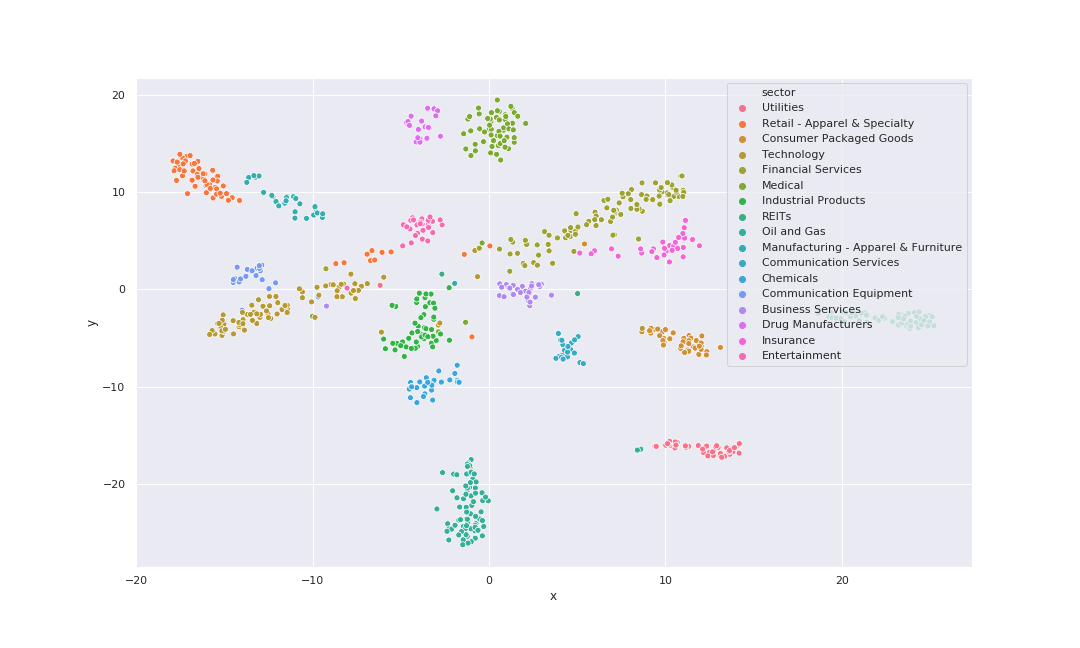
\includegraphics[height=\textheight]{./figures/tsne.png}
    \caption{T-SNE of the embedding layers of the network.}
    \end{center}
  \end{figure}

  \begin{figure}    
  \begin{center}
    \label{fig:silhouette-score}
    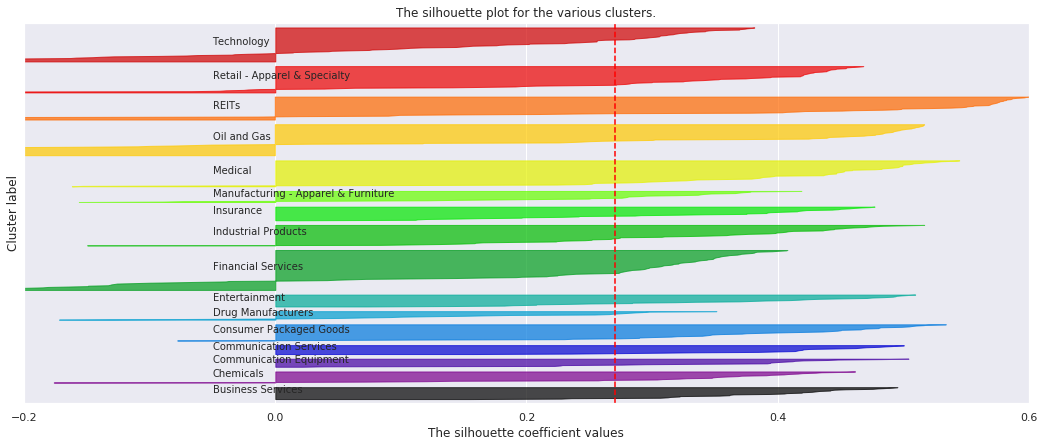
\includegraphics[height=\textheight]{./figures/silouhette_score}
    \caption{Silouhette score of the average embedding of the stocks}
    \end{center}
  \end{figure}
\end{landscape}

In Figure \ref{fig:silhouette-score}, the silouhette score is depicted for the
several sectors in our dataset. The first observation is we see the advantage
of a neural network classifier over k-means clustering, because the silhouette
score overweights the mislabeled sample of financial and technology, which are
the most precise sectors. Otherwise we can observe that REiTS, Oil and Gas,
and the Insurance sector are grouped tightly making them quite distinct group.


\section{Conclusion and Further applications}
\label{sec:orgc4d755f}

The first lesson I learned is data preparation and acquisition is much harder
than thought and we should thank the machine learning community for providing
so many labeled data set for our development. Indeed the financial industry
still leverage on providing exclusive data and create a difficult task to
leverage on alternative dataset, which could potentially provide added value.

Second, in deep learning, a bigger network does not necessarily translate into
a better performance: training is much more difficult with more parameters
even with regularizers and advanced optimization method.

However, these most so-called quantitative strategies require data in the most
accurate form and event the most trusted data provider fails to deliver the
data without flaws.

Inconvenient: for now it is impossible to detect new group in as we would need
to train them. Zero shot learning would be an interesting project to the
study.
\end{document}